\section{Соизмеримые и несоизмеримые отрезки}

\begin{wrapfigure}{r}{37mm}
\centering
\includegraphics{mppics/ris-162}
\caption{}\label{1938/ris-162}
\end{wrapfigure}

\paragraph{Общая мера.}\label{1938/145}\rindex{общая мера}
Общей мерой двух отрезков называется такой третий отрезок, который в каждом из первых двух содержится целое число раз без остатка.
Так, если отрезок $AM$ (рис.~\ref{1938/ris-162}) содержится 5 раз в $AB$ и 3 раза в $CD$, то $AM$ есть общая мера $AB$ и $CD$.
Подобно этому можно говорить об общей мере двух дуг одинакового радиуса, двух углов и вообще двух однородных величин.

{\small
\smallskip
\so{Замечание}.
Очевидно, что если отрезок $AM$ есть общая мера
отрезков $AB$ и $CD$, то, разделив $AM$ на 2, 3, 4 и так далее равные
части, мы получим меньшие общие меры для отрезков $AB$ и $CD$.
Таким образом, если два отрезка имеют какую-нибудь общую меру, то можно сказать, что они имеют бесчисленное множество общих мер.
Одна из них будет наибольшая.
}

\paragraph{Теоремы о наибольшей общей мере.}\label{1938/146}
Чтобы найти наибольшую общую меру двух отрезков, употребляют так называемый \rindex{алгоритм Евклида}\textbf{алгоритм Евклида} — способ последовательного отложения, подобный тому последовательному делению, каким в арифметике находят наибольший общий делитель двух целых чисел. 

Этот способ основывается на следующих теоремах.

\begin{wrapfigure}{o}{24mm}
\centering
\includegraphics{mppics/ris-163}
\caption{}\label{1938/ris-163}
\end{wrapfigure}

1.
\textbf{\emph{Если меньший из двух отрезков}} ($a$ и $b$, рис.~\ref{1938/ris-163}) \textbf{\emph{содержится в большем целое число раз без остатка, то наибольшая общая мера этих отрезков есть меньший из них.}}

Пусть, например, отрезок $b$ содержится в отрезке $a$ ровно $3$ раза;
так как при этом, конечно, отрезок $b$ содержится в самом себе ровно $1$ раз, то $b$ есть общая мера отрезков $a$ и $b$;
с другой стороны, эта мера есть и наибольшая, так как никакой отрезок, больший $b$, не может содержаться в $b$ целое число раз.

2.
\textbf{\emph{Если меньший из двух отрезков}} ($b$, рис.~\ref{1938/ris-164}) \textbf{\emph{содержится в большем}} ($a$) \textbf{\emph{целое число раз с некоторым остатком}} ($r$), \textbf{\emph{то наибольшая общая мера этих отрезков}} (если она существует) \textbf{\emph{должна быть и наибольшей общей мерой меньшего отрезка}} ($b$) \textbf{\emph{и остатка}} ($r$).

\begin{wrapfigure}{O}{30mm}
\centering
\includegraphics{mppics/ris-164}
\caption{}\label{1938/ris-164}
\end{wrapfigure}

Пусть, например.
\[a=b+b+b+r.\]
Из этого равенства мы можем вывести следующие два заключения.

1) Если существует отрезок, содержащийся без остатка в $b$ и $r$, то он содержится также без остатка и в $a$;
если, например, какой-нибудь отрезок содержится в $b$ ровно 5 раз и в $r$ содержится ровно 2 раза, то в $a$ он содержится 5 + 5 + 5 + 2, то есть 17 раз без остатка.

2) Обратно:
если существует отрезок, содержащийся без остатка в $a$ и $b$, то он содержится также без остатка и в $r$;
если, например, какой-нибудь отрезок содержится в $a$ ровно 17 раз и в $b$ ровно 5 раз, то в той части отрезка $a$, которая равна $3b$, он содержится 15 раз;
следовательно, в остающейся части отрезка $a$, то есть в $r$, он содержится $17-15$, то есть 2 раза.

Таким образом, у двух пар отрезков
\[\overbrace{a\ \text{и}\ b},\quad \overbrace{b\ \text{и}\ r}\]
должны быть одни и те же общие меры (если они существуют);
поэтому и \so{наибольшая} общая мера у них должна быть одна и та же.
К этим двум теоремам надо ещё добавить следующую \rindex{аксиома!измерения}\textbf{аксиому измерения} (так называемую \rindex{аксиома!Архимеда}аксиому Архимеда). 

\textbf{\emph{Как бы велик ни был больший отрезок}} ($a$) \textbf{\emph{и как бы мал ни был меньший отрезок}} ($b$), \textbf{\emph{всегда, откладывая меньший на большем последовательно 1, 2, 3 и так далее раз, мы получим, что после некоторого $\bm{m}$-го отложения или не получится никакого остатка, или получится остаток, меньший меньшего отрезка}} ($b$);
другими словами, всегда можно найдётся достаточно большое целое положительное число $m$, что $b \cdot  m \le a$, но $b \cdot  (m + 1) > a$. 

\paragraph{Алгоритм Евклида.}\label{1938/147}
Пусть требуется найти наибольшую общую меру двух данных отрезков $AB$ и $CD$ (рис.~\ref{1938/ris-165}).

\begin{wrapfigure}{o}{48mm}
\centering
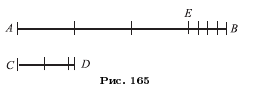
\includegraphics{mppics/ris-165}
\caption{}\label{1938/ris-165}
\end{wrapfigure}

Для этого на большем отрезке откладываем (с помощью циркуля) меньший отрезок столько раз, сколько это возможно.
При этом, согласно аксиоме измерения, случится одно из двух:
или 
1) $CD$ уложится в $AB$ без остатка, тогда искомая мера, согласно теореме 1, будет $CD$, 
или 2) получится некоторый остаток $EB$, меньший $CD$ (как у нас на чертеже);
тогда, согласно теореме 2, вопрос приведётся к нахождению наибольшей общей меры двух меньших отрезков, именно $CD$ и первого остатка $EB$.
Чтобы найти её, поступаем точно так же, то есть откладываем $EB$ на $CD$ столько раз, сколько можно.
И опять произойдёт одно из двух:
или 1) $EB$ уложится в $CD$ без остатка, тогда искомая мера и будет $EB$, 
или 2) получится остаток $FD$, меньший $EB$ (как у нас на чертеже);
тогда вопрос приведётся к нахождению наибольшей общей меры двух меньших отрезков, именно $EB$ и второго остатка $FD$.

Продолжая этот приём далее, мы можем встретиться с такими двумя возможными случаями:

1) после некоторого отложения не получится никакого остатка или

2) процесс последовательного отложения не будет иметь конца (в предположении, что мы имеем возможность откладывать как угодно малые отрезки, что, конечно, возможно только теоретически).

В первом случае последний остаток и будет наибольшей общей мерой данных отрезков.
Чтобы удобней вычислить, сколько раз эта наибольшая общая мера содержится в данных отрезках, выписываем ряд равенств, получаемых после каждого отложения.
Так, по нашему чертежу мы будем иметь:
\begin{align*}
&\text{после}
&&\text{первого}
&\text{отложения}&:
&AB &= 3\cdot CD + EB;
\\
&\text{\ —\textquotedbl—}
&&\text{второго}
&\text{—\textquotedbl—\ \ \ \ }&:
&CD &= 2\cdot EB + FD;
\\
&\text{\ —\textquotedbl—}
&&\text{третьего}
&\text{—\textquotedbl—\ \ \ \ }&:
&EB &= 4\cdot FD.
\end{align*}
Переходя в этих равенствах от нижнего к верхнему, последовательно находим:
\begin{align*}
EB&=4\cdot FD;
\\
CD&=(4\cdot FD)\cdot 2+FD=9\cdot FD;
\\
AB&=(9\cdot FD)\cdot 3+4\cdot FD=31\cdot FD.
\end{align*}
Подобно этому можно находить наибольшую общую меру двух дуг одинакового радиуса, а также двух углов.

\smallskip
\so{Во втором} случае данные отрезки не могут иметь общей меры.
Чтобы обнаружить это, предположим, что данные отрезки $AB$ и $CD$ имеют какую-нибудь общую меру.
Мера эта, как мы видели, должна содержаться целое число раз не только в $AB$ и в $CD$, но и в остатке $EB$, следовательно, и во втором остатке $FD$, и в третьем, и в четвёртом и~т.~д.
Так как остатки эти идут, последовательно уменьшаясь, то в каждом из них общая мера должна содержаться меньшее число раз, чем в предыдущем остатке.
Если, например, в $EB$ общая мера содержится $100$ раз (вообще $m$ раз), то в $FD$ она содержится менее $100$ раз (значит, не более $99$ раз);
в следующем остатке она должна содержаться менее $99$ раз (значит, не более $98$ раз) и~т.~д.
Так как ряд целых положительных уменьшающихся чисел:
$100, 99, 98, \dots$
(и вообще $m, m-1, m-2,\dots$) имеет конец (как бы велико ни было число $m$), то и процесс последовательного отложения, при достаточном его продолжении, должен дойти до конца, то есть мы дойдём до того, что уже не получится никакого остатка.
Значит, если последовательное отложение не имеет конца, то данные отрезки никакой общей меры иметь не могут.

\paragraph{Соизмеримые и несоизмеримые отрезки.}\label{1938/148}\rindex{соизмеримые отрезки}\rindex{несоизмеримые отрезки}
Два отрезка называются соизмеримыми, если они имеют общую меру, и несоизмеримыми, когда такой общей меры не существует.

На практике нет возможности убедиться в существовании несоизмеримых отрезков, потому что, продолжая последовательное отложение, мы всегда дойдём до столь малого остатка, который в предыдущем остатке, по-видимому, укладывается целое число раз.
Быть может при этом и должен был бы получиться некоторый остаток, но по причине неточности инструментов (циркуля) и несовершенства наших органов чувств (зрения) мы не в состоянии его заметить.
Однако, как мы сейчас докажем, несоизмеримые отрезки существуют.

{\small

\paragraph{}\label{1914/156}
\so{Теорема}.
\textbf{\emph{Если в равнобедренном треугольнике угол при основании равен $\bm{36\degree}$, то боковая сторона его несоизмерима с основанием.}}

Пусть $ABC$ равнобедренный треугольник (рис.~\ref{1914/ris-147}), у которого каждый из углов $A$ и $C$ равен $36\degree$; 
требуется доказать, что боковая сторона $AB$ несоизмерима с основанием $AC$.

\begin{wrapfigure}{o}{48mm}
\centering
\includegraphics{mppics/ris-1914-147}
\caption{}\label{1914/ris-147}
\end{wrapfigure}

Прежде всего определим, которая из этих сторон больше.
Для этого достаточно сравнить углы, против которых лежат эти стороны.
Так как, по условию, $\angle A=\angle C\z=36\degree$, то 
\[\angle B=180\degree-36\degree-36\degree=108\degree;\]
следовательно, $\angle B>\angle C$;
поэтому $AC\z>AB$.

Теперь найдём сколько раз в $AC$ уложиться $AB$.
Так как $AC\z<AB+BC$ и $AB=BC$ то $AC<2\cdot AB$;
значит $AB$ может уложиться только один раз с некоторым остатком.

Таким образом, мы замечаем следующее свойство:
\emph{если в равнобедренном треугольнике угол при основании равен $36\degree$, то боковая его сторона содержится в основании только один раз и притом с некоторым остатком.}

Заметив это, приступим к последовательному отложению.
Отложим на $AC$ часть $AD$, равную $AB$ тогда получим остаток $DC$, который надо накладывать на $AB$, или, что все равно, на $BC$.

Чтобы узнать, сколько раз $DC$ уложится на $BC$, соединим $B$ с $D$ и рассмотрим $\triangle DBC$.
Найдём его углы.
Так как $\triangle ABD$ равнобедренный, то $\angle ABD = \angle ADB$;
следовательно, каждый из них равен 
\[\tfrac12(180\degree -\angle A)=\tfrac12(180\degree -36\degree)=72\degree.\]
Но угол $ABC$, как мы прежде нашли, равен $108\degree$; следовательно, 
\[\angle DBC=108\degree-72\degree=36\degree.\]
Таким образом, в треугольнике $DBC$ есть два равных угла при $BC$; следовательно, он равнобедренный, при чем каждый угол при его основании $BC$ равен $36\degree$.

Вследствие этого, по доказанному выше, боковая сторона его $DC$
(или $BD$) уложится в основании $BC$ \emph{один раз с некоторым остатком}.
Пусть этот остаток будет $EC$.
Соединив $E$ с $D$, мы снова получим равнобедренный треугольник $CDE$, в котором каждый угол при основании $CD$ равен $36\degree$.
Отложив $EC$ (или $DE$) на $DC$ (от точки $D$), мы снова получим равнобедренный треугольник $CEF$, у которого каждый угол при основании $CE$ равен $36\degree$.

Таким образом, мы постоянно будем приходить к равнобедренному треугольнику (всё меньшему и меньшему) с углами при основании, равными $36\degree$;
следовательно, мы никогда в этом процессе \so{не дойдём до конца}.
Значит, стороны $AC$ и $AB$ не могут иметь общей меры.

{\small

\smallskip
{\so{Примечание}.}
Первый пример несоизмеримых отрезков приписывается пифагорейцу Гиппасу из Метапонта (приблизительно 470 год до нашей эры).
Есть основания полагать, что Гиппас доказал несоизмеримость стороны и диагонали правильного пятиугольника, хотя сколько-нибудь уверенных подтверждений тому нет.
Нетрудно видеть что треугольник отсекаемый диагональю от правильного пятиугольника равнобедренных и имеет углы при основании равные $36\degree$.
То есть возможно приведённое построение повторяет то, что было сделано Гиппасом.

}

\paragraph{}\label{1938/149}
\so{Теорема}.
\textbf{\emph{Диагональ квадрата несоизмерима с его стороной.}}

\begin{wrapfigure}{o}{42mm}
\centering
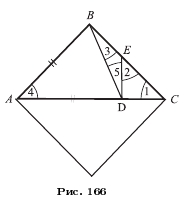
\includegraphics{mppics/ris-166}
\caption{}\label{1938/ris-166}
\end{wrapfigure}

Так как диагональ делит квадрат на два равнобедренных прямоугольных треугольника, то теорему эту можно высказать иными словами так:
\textbf{\emph{гипотенуза равнобедренного прямоугольного треугольника несоизмерима с его катетом.}}

Предварительно докажем следующее свойство такого треугольника;
если на гипотенузе (рис.~\ref{1938/ris-166}) отложим отрезок $AD$, равный катету, и проведём $DE\perp AC$, то образовавшийся при этом прямоугольный треугольник $DEC$ будет равнобедренный, а отрезок $BE$ катета $BC$ окажется равным отрезку $DC$ гипотенузы.
Чтобы убедиться в этом, проведём прямую $BD$ и рассмотрим углы треугольников $DEC$ и $BED$.
Так как треугольник $ABC$ равнобедренный и прямоугольный, то $\angle 1 \z= \angle 4$, и, следовательно, $\angle 1 \z= 45\degree$, а потому в прямоугольном треугольнике $DEC$ и $\angle 2 = 45\degree$ и, значит, треугольник $DEC$ имеет два равных угла и потому его стороны $DC$ и $DE$ равны.



В треугольнике $BDE$ угол 3 равен прямому углу $B$ без угла $ABD$, а угол 5 равен прямому углу $ABE$ без угла $ABD$.
Но $\angle ADB \z= \angle ABD$ (так как $AB=AD$);
значит, и $\angle 3 = \angle 5$.
Но тогда треугольник $BDE$ должен быть равнобедренный, и потому $BE=ED=DC$.

Заметив это, станем находить общую меру отрезков $AB$ и $AC$.

Так как $AC>AB$ и $AC<AB+BC$, то есть
$AC<2AB$, то катет $AB$ отложится на гипотенузе $AC$ только один раз с некоторым остатком $DC$.
Теперь надо этот остаток откладывать на $AB$ или, что всё равно, на $BC$.
Но отрезок $BE$, по доказанному, равен $BC$.
Значит, надо $BC$ отложить ещё на $EC$.
Но $EC$ есть гипотенуза равнобедренного треугольника $DEC$.
Следовательно, процесс отложения для нахождения общей меры сводится теперь к откладыванию катета $BC$ прямоугольного равнобедренного треугольника $DEC$ на его гипотенузе $EC$.
В свою очередь это отложение сведётся к откладыванию катета на гипотенузе нового меньшего прямоугольного равнобедренного треугольника и~т.~д., очевидно, без конца.
А если процесс этот не может окончиться, то общей меры отрезков $AC$ и $AB$ не существует.

\paragraph{Цепные дроби.}\label{extra/tzepnye-drobi}
В дополнение к десятичным дробям мы рассмотрим другой способ который позволяют записать число.
Он основан на последовательности частных полученных в алгоритме Евклида (§~\ref{1938/147}).
Этот способ записи не удобен для складывания и умножения чисел, но очень удобен для отыскания приближений числа в виде дробей с небольшими знаменателями.

{

\begin{wrapfigure}{r}{48mm}
\vskip0mm
\centering
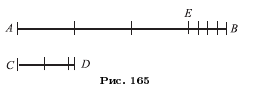
\includegraphics{mppics/ris-165}
\caption{}\label{1938/ris-165-1}
\bigskip
\includegraphics{mppics/ris-extra-7}
\caption{}\label{extra/ris-7}
\bigskip
\includegraphics{mppics/ris-extra-8}
\caption{}\label{extra/ris-8} 
\end{wrapfigure}

Вычисление отношения отрезков $\frac{AB}{CD}\z=\frac{31}{9}$ (рис.~\ref{1938/ris-165-1}) данное в §~\ref{1938/147},
можно компактно записать следующим образом:
\begin{align*}
\frac{AB}{CD}&=3+\frac{EB}{CD}=3+\frac{1}{\frac{CD}{EB}}=
\\
&=3+\frac{1}{2+\frac{FD}{EB}}=3+\frac{1}{2+\frac{1}{\frac{EB}{FD}}}
\\
&=3+\frac{1}{2+\frac{1}{4}}.
\end{align*}

Последнее выражение называется \rindex{цепная дробь}\textbf{цепной дробью}.
В этом случае процесс построения цепной дроби оборвался на третьем шаге, так как отрезок $FD$ вмещается 4 раза в $EB$ без остатка.
Вообще, любое рациональное число представляется конечной цепной дробью.

Для несоизмеримых отрезков этот процесс можно было бы продолжать сколь угодно долго получая всё более длинные дроби.


Например для пары отрезков $AC$ и $AB$ в (§~\ref{1914/156}) мы получим бесконечную цепную дробь составленную из одних единиц: 
\begin{align*}
\frac{AC}{AB}&=1+\frac{DC}{AB}=1+\frac1{\frac{AB}{DC}}=
\\
&=1+\frac1{1+\frac{EC}{DC}}=1+\frac1{1+\frac1{\frac{DC}{EC}}}=
\\
&=\cdots=1+\frac1{1+\frac1{1+\cdots}}
\end{align*}

}

Из доказательства в §~\ref{1938/149} следует, что для отношения диагонали квадрата к его стороне получается цепная дробь из двоек:
\[\alpha=1+\frac1{2+\frac1{2+\cdots}}.\eqno(1)\]
Из теоремы Пифагора доказанной ниже (§~\ref{1938/191}) следует, что $\alpha\z=\sqrt2$;
но это же можно увидеть непосредственно: в знаменателе выражения для $\alpha$ мы копию $\alpha$ плюс один; то есть 
$\alpha=1+\frac1{1+\alpha}$ и значит $\alpha^2=2$.



Для нахождения приближений числа с небольшим знаменателем,
достаточно оборвать цепную дробь и привести её к обычному виду.
Такие дроби называются \rindex{подходящая дробь}\textbf{подходящими}.
Например для $\sqrt2$ мы получаем следующие приближения:
\[1,\quad \tfrac 32=1+\tfrac12,\quad \tfrac75=1+\frac1{2+\frac12},\quad \tfrac{17}{12}=1+\frac1{2+\frac1{2+\frac12}},\quad \dots\]
Несложно проверить, что нечётные подходящие дроби дают приближение с недостатком, а чётные с избытком.
При этом оказывается, что подходящие дроби являются \so{лучшими} приближениями среди всех дробей с меньшими знаменателями.

\paragraph{О теории пропорций.}\label{extra/evdox}
В современной математике уравнение $\frac{a}{b}\z=\frac{c}{d}$
для длин $a$, $b$, $c$ и $d$ четырёх отрезков  понимается как равенство двух вещественных чисел, каждое из них отношение пары вещественных чисел.

Во времена Евклида, под числом понимались только положительные рациональные числа.
Длины же отрезков и промежутки времени назывались \rindex{величина}\textbf{величинами} и числом не считались.
Как мы знаем, 
если выбрана единица измерения (например секунда для времени или метр для длины), то величину можно выразить вещественным числом; но во времена Евклида это не было известно.

Величины одного рода можно было сравнивать, складывать и умножать на натуральное число. 
Чтобы делить или умножать одну величину на другую пользовались специальными приёмами;
например про произведение двух длин думали как про площадь прямоугольника с данными сторонами.
Была также развита теория пропорций по-сути позволяющая делить одну величину на другую.

Для того чтобы выразить уравнение $\frac{a}{b}=\frac{c}{d}$, говорили «$a$ относится к $b$ также как $c$ относится к $d$».
Изначально это выражение означало, что цепная дробь получаемая при делении $a$ на $b$ в точности совпадает с цепной дробью при делении $c$ на $d$.
Иначе говоря, если применить алгоритм Евклида (§~\ref{1938/147}) к паре отрезков $a$ и $b$ то полученные частные будут в точности те же, что и для пары $c$ и $d$.

Позже Евдокс (живший в IV веке до нашей эры) дал следующее, более удобное определение, равносильное следующему: \emph{$a$ относится к $b$ также как $c$ относится к $d$ если для любых натуральных чисел $m$ и $n$ верно одно из трёх утверждений:
\begin{align*}
\text{либо}\quad m\cdot a&>n\cdot b\quad\text{и}\quad m\cdot c>n\cdot d,
\\
\text{либо}\quad m\cdot a&=n\cdot b\quad\text{и}\quad m\cdot c=n\cdot d,
\\
\text{либо}\quad m\cdot a&<n\cdot b\quad\text{и}\quad m\cdot c<n\cdot d.
\end{align*}
}
Это определение было включено в «Начала» Евклида.

Позже определение Евдокса было использовано немецким математиком Рихардом Дедекиндом для того чтобы дать точное определение вещественных чисел;
сегодня его определение считается основным.
Поскольку учащиеся знакомы с десятичными дробями, мы использовали их как определение вещественных чисел, но строгий вывод всех необходимых свойств десятичных дробей несоизмеримо сложней чем при подходе  Евдокса и Дедекинда.

}
